\documentclass[10pt,titlepage]{article}
\usepackage[english]{babel}
\usepackage[utf8]{inputenc}
\usepackage{algorithm}
\usepackage[noend]{algpseudocode}
\usepackage{amsmath,amsfonts,amsthm}
\usepackage{spverbatim}
\usepackage{listings}
\usepackage{xcolor}
\usepackage{pgfplots}
\usepackage[letterpaper, margin=1.25in]{geometry}
\usepackage{titlesec}
\usepackage{fancyhdr}
\usepackage{graphicx}
\usetikzlibrary{trees}
\usepackage[normalem]{ulem}
\useunder{\uline}{\ul}{}

\lstdefinestyle{mystyle}{
	keywordstyle=\color{blue},
	commentstyle=\color{red},
	stringstyle=\color{violet},
	basicstyle=\fontsize{12}{12},
	columns=fullflexible,
	breaklines=true
}

\titleformat{\section}
{\normalfont\Large\bfseries}{\thesection}{1em}{}[{\titlerule[0.8pt]}]
\lstset{style=mystyle}

\title{High Level Design}

\author{Seth Williams, Abraham Sharum, Parker Fletcher, Bryson Dye \\\\ \\ Due Date: September 11, 2025 \\ Class: CS 40003 - Software Engineering}	

\lstset{style=mystyle}
\begin{document}
	\pagestyle{fancy}
	\fancyhead{}
	\fancyhead[LE,LO]{\textbf{CS 40003 - Software Engineering}}
	\fancyhead[RO,RE]{\textbf{High Level Desgin}}
	\fancyfoot{}
	\fancyfoot[CE,CO]{\textbf{\thepage}}
	\maketitle
	
	\section*{Data Flow Diagram}

    \begin{figure}[H]
    	\centering
    	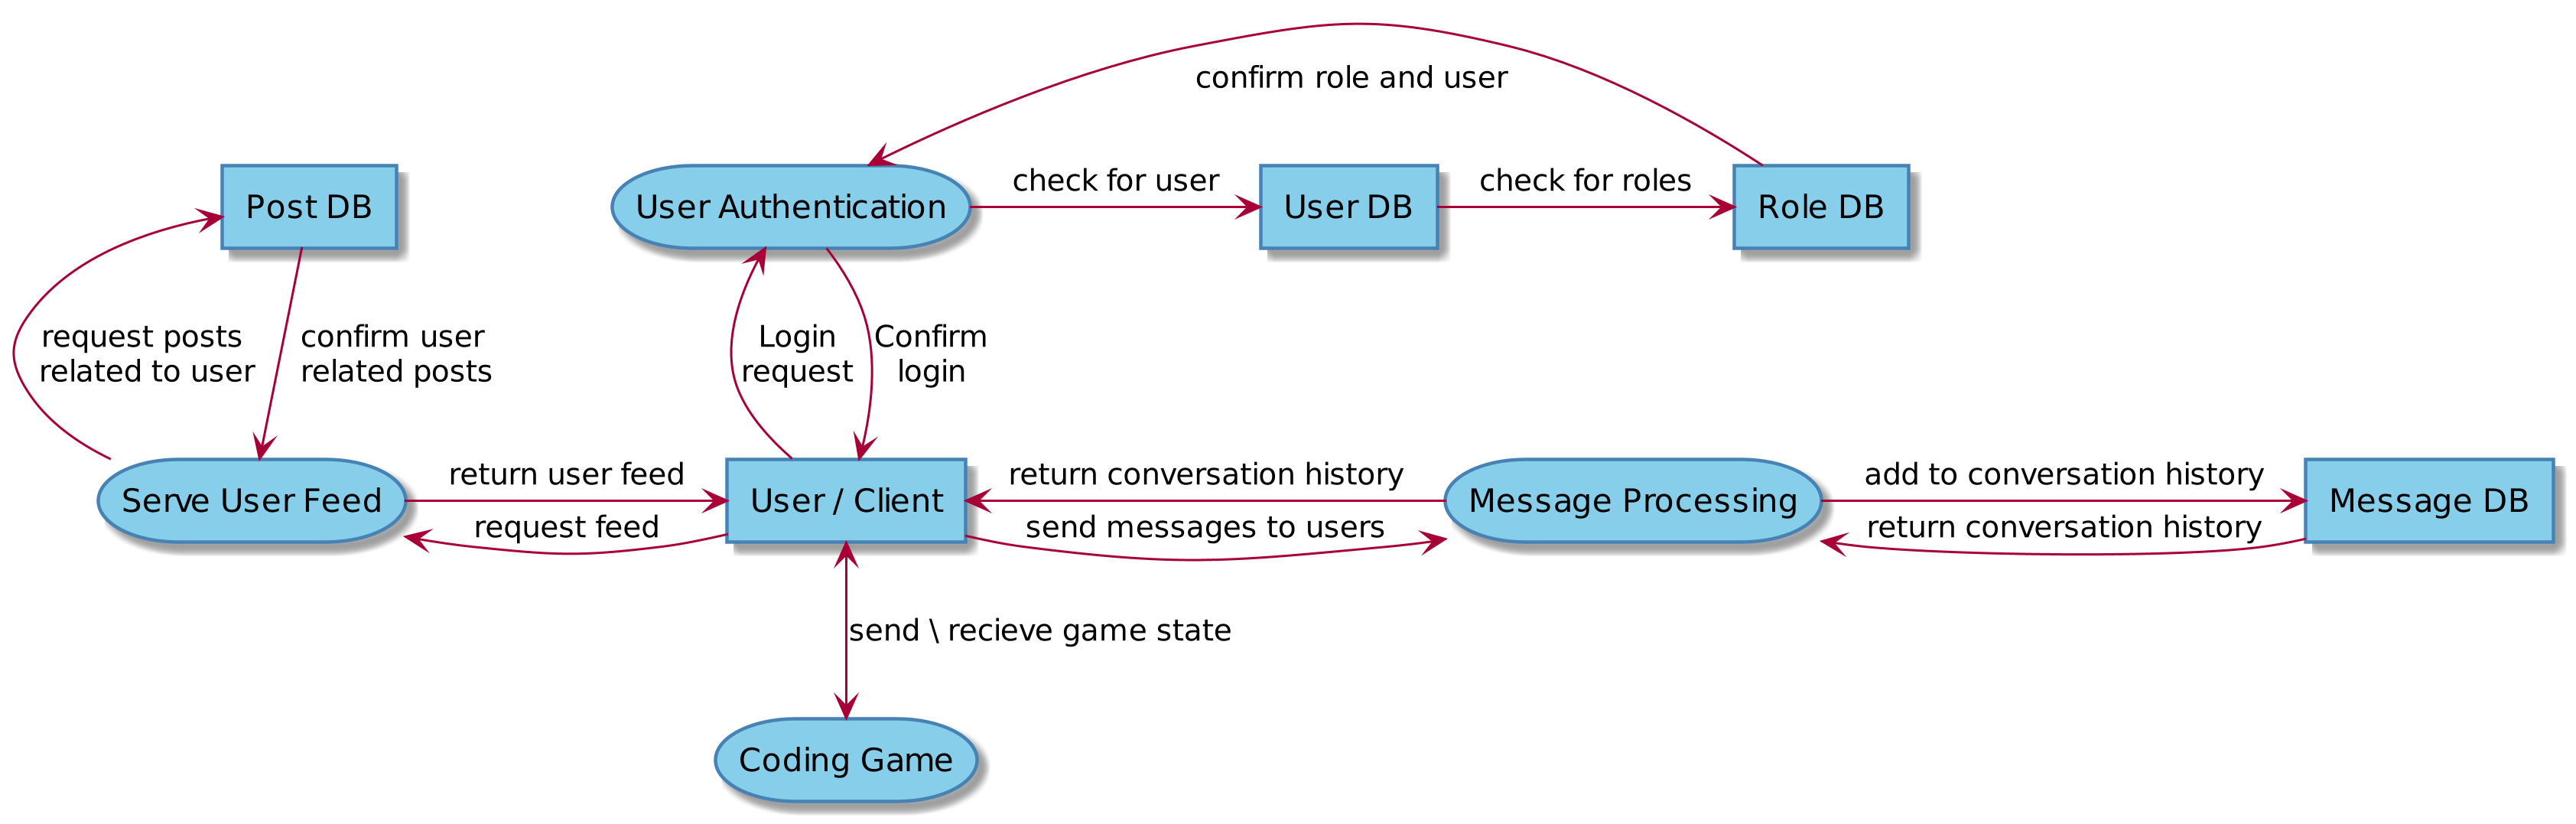
\includegraphics[width=1\textwidth]{DataFlowDiagram.png}
    	\caption{Data Flow Diagram}
    	\label{fig:dataflow}
	\end{figure}
	
	\section*{Deployment Diagram}
	
	\begin{figure}[H]
		\centering
		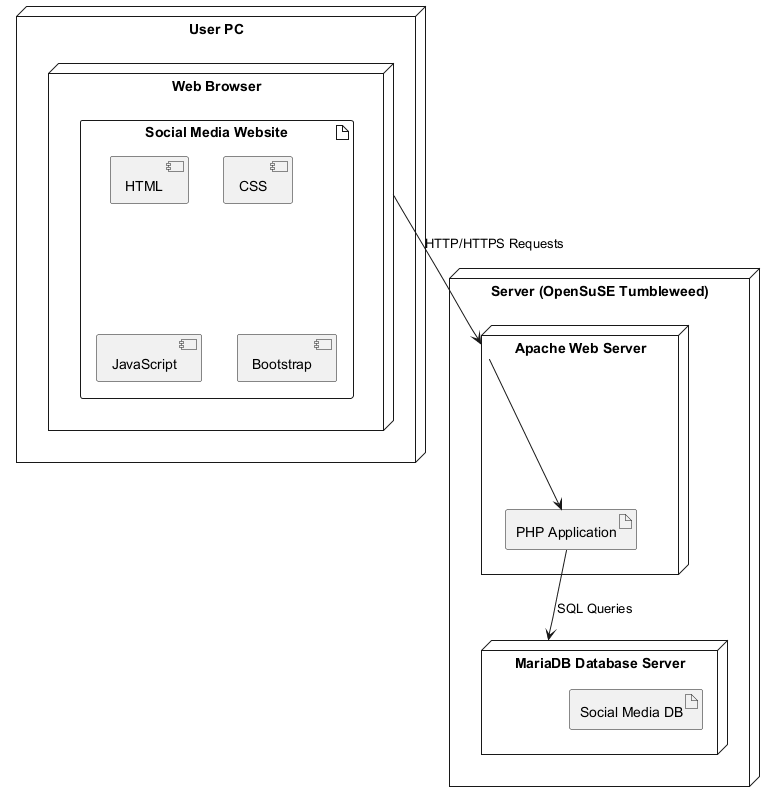
\includegraphics[width=1\textwidth]{DeploymentDiagram.png}
		\caption{Deployment Diagram}
		\label{fig:deployment}
	\end{figure}
	
	\section*{System Architecture Diagram}
	
	\begin{figure}[H]
		\centering
		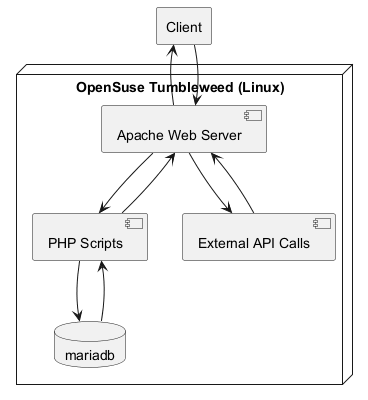
\includegraphics[width=1\textwidth]{SystemArchi.png}
		\caption{System Architecture Diagram}
		\label{fig:systemArch}
	\end{figure}
	
	\section*{Tech Stack}
	
	\begin{figure}[H]
		\centering
		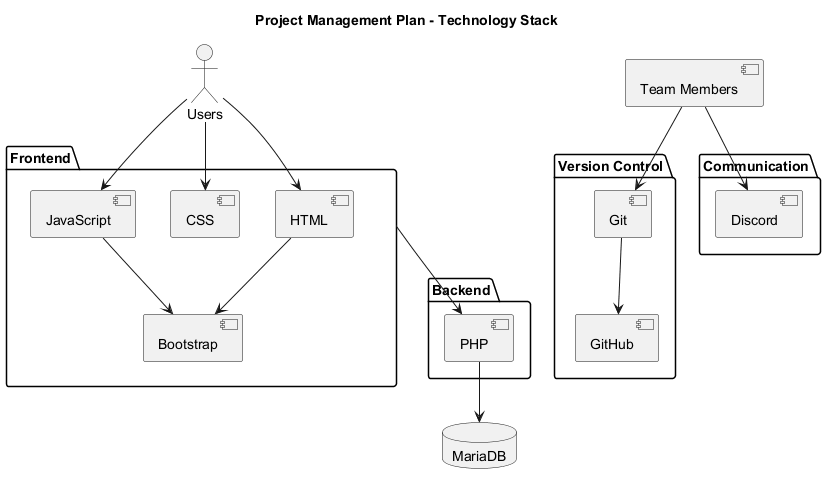
\includegraphics[width=1\textwidth]{Tech Stack.png}
		\caption{Tech Stack Diagram}
		\label{fig:techStack}
	\end{figure}

	
\end{document}
